\documentclass{beamer}

\title{Hashtables}

\usepackage{listings,graphicx}
\lstset{language=Ruby,basicstyle=\small}

\subtitle{Lunch \& Learn}
\author{Ethan Kent}
\date{\today}
\subject{Computer Science}

\begin{document}
\frame{\titlepage}

\begin{frame}
    \frametitle{Purpose}

    The goal of this presentation is to discuss what hashtables are, how they
    work, and the tradeoffs that go along with different designs.
\end{frame}

\begin{frame}[fragile]
    \frametitle{Data structures and tradeoffs}
    \framesubtitle{Linked lists}

    \texttt{O(1)} insertion and popping; \texttt{O(n)} for search, access by
    position.

    \begin{lstlisting}
Node = Struct.new(:value, :next_node)

node1 =  Node.new(0)
node2 =  Node.new(1)
node3 =  Node.new(2)
node4 =  Node.new(3)

node1.next_node = node2
node2.next_node = node3
node3.next_node = node4
node4.next_node = :null_pointer

puts node1
    \end{lstlisting}
\end{frame}

\begin{frame}[fragile]
    \frametitle{Data structures and tradeoffs}
    \framesubtitle{Arrays}

    Linked lists have pointers to arbitrary other locations in memory. By
    contrast, arrays are contiguous locations in memory.

    \vspace{1em}

    Arrays have \texttt{O(1)} insertion, popping, and access by position, and
    \texttt{O(n)} search.

    \begin{lstlisting}[language=C]
int * my_array;

my_array = (int * ) malloc(sizeof(int) * 50);

for(i = 0; i < 50; ++i) {
    my_array[i] = 0;
}
    \end{lstlisting}

\end{frame}

\begin{frame}
    \frametitle{Data structures and tradeoffs}
    \framesubtitle{The desire for constant-time ``find'' operations}

    \begin{itemize}
        \item With a linked list, we can only find an element by starting at
              the beginning and searching every spot. We can't even go directly to
              an element if we know its index.
        \item With a vector, we can only find an element by starting at the
              beginning and searching every spot. But we \emph{can} go
              directly to an element if we know its index.
    \end{itemize}

    \vspace{1em}

    It would be nice would be to have some way to use the value we're
    checking for \emph{to tell us where to look}, so we could go directly
    there.
\end{frame}

\begin{frame}
    \frametitle{An analogy}
    What if we had a machine that could use the description of your backpack:

    \begin{center}
        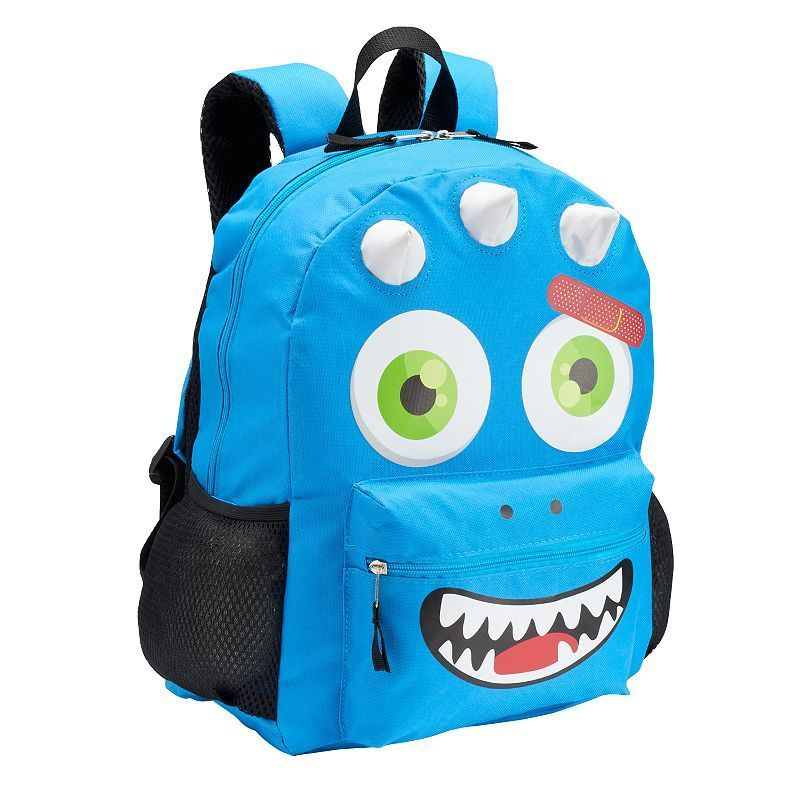
\includegraphics[height=0.3\textheight]{backpack.jpg}
    \end{center}

    and tell you it belongs in locker 57?

    \begin{center}
        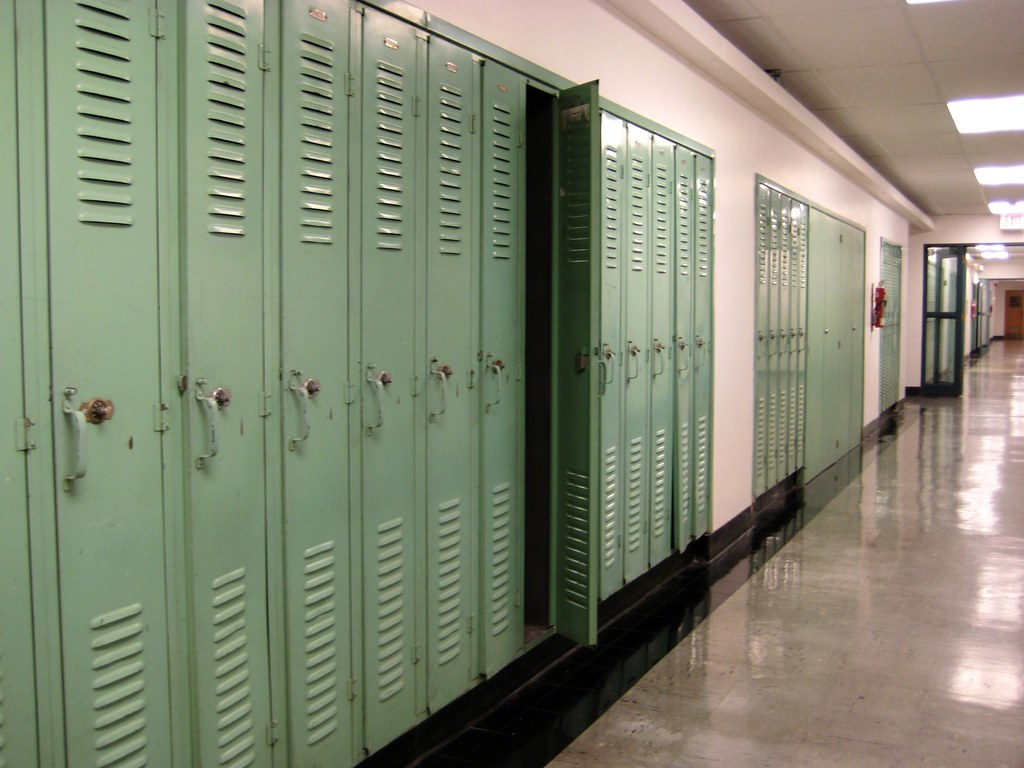
\includegraphics[width=0.3\textheight]{lockers.jpg}
    \end{center}
\end{frame}

\begin{frame}
    \frametitle{An analogy}

    What else would our machine have to do? It should---

    \begin{itemize}
        \item Always give you the same answer given the same backpack.
        \item Not put every backpack in locker 57.
        \item Not put most backpacks in just a few lockers.
        \item Not put most blue backpacks in just a few lockers.
        \item Give you an answer pretty quickly.
    \end{itemize}

    \vspace{1em}

    If we had that, we could walk directly do locker 57 and get our backpack,
    without the need to search.
\end{frame}

\begin{frame}
    \frametitle{An analogy}
    \begin{center}
        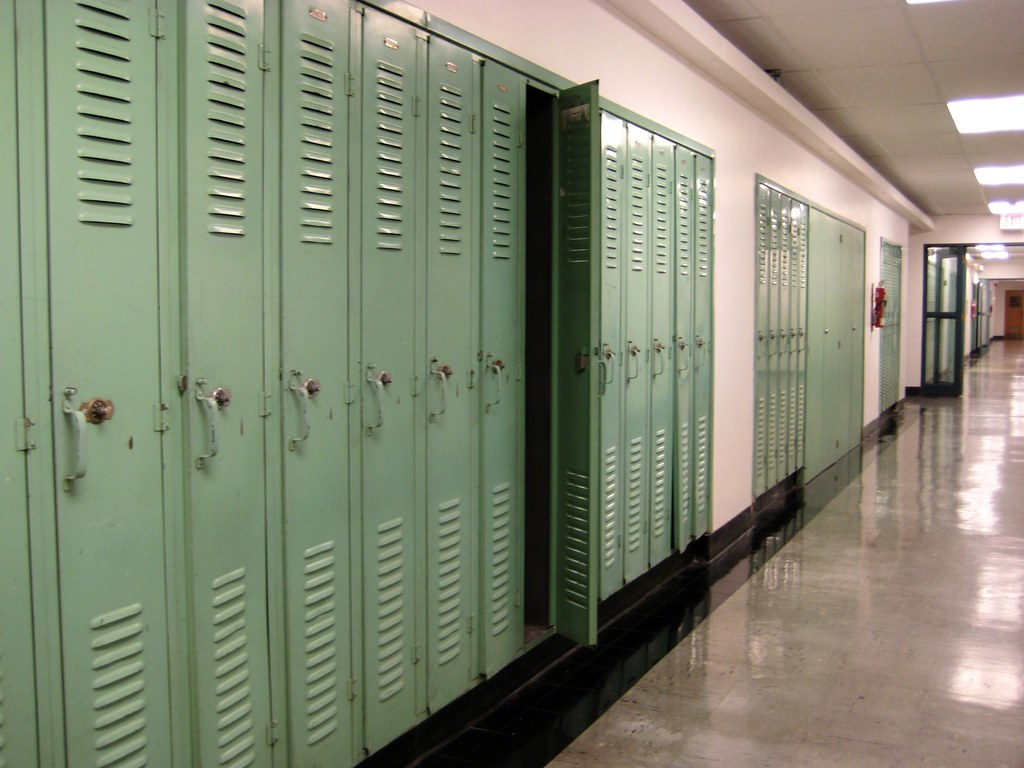
\includegraphics[width=0.5\textheight]{lockers.jpg}
    \end{center}

    But there are still some problems. What if---

    \begin{itemize}
        \item More than one backpack is assigned to the same locker (assume
              only one backpack can fit)?
        \item There are more backpacks than lockers?
    \end{itemize}
\end{frame}

\begin{frame}
    \frametitle{Hashtables}
    We have now considered several aspects of a data structure called a
    \emph{hashtable}.

    \vspace{1em}

    \begin{itemize}
        \item The machine that turns the backpack into a locker assignment is
              a hash function.
        \item The characteristics of a good backpack assigner are the
              characteristics of a good hash function:
              \begin{itemize}
                  \item Deterministic,
                  \item Fast,
                  \item Uniform, and
                  \item Avalanching.
              \end{itemize}
        \item The problems you can run into are the same as those with a hashtable:
              \begin{itemize}
                  \item Collisions, and
                  \item Load factor.
              \end{itemize}
    \end{itemize}
\end{frame}

\begin{frame}
    \frametitle{The key idea}

    If we can use \emph{the data itself} to tell us where the data belongs,
    and if we can go directly to where the data belongs, we get best-case
    \texttt{O(1)}. This compares favorably with:

    \vspace{1em}

    \begin{itemize}
        \item Fully sorting the data (\texttt{O(n log n)} for insertion).
        \item Traversing a linked list or array (\texttt{O(n)} for search).
        \item Using a balanced data structure (\texttt{O(log n)} for common
              operations).
    \end{itemize}
\end{frame}

\begin{frame}
    \frametitle{The birthday problem}

    You're throwing a party. You invite one person at a time until two people
    have the same birthday. On average, how many people do you have to invite
    to your party (assuming birthdays are distributed evenly across a 365-day
    year?)
\end{frame}

\begin{frame}[fragile]
    \frametitle{The birthday problem}
    \begin{lstlisting}
require "set"
year = (1..365).to_a
num_runs = 100_000

total = num_runs.times.reduce(0.0) do |total|
  set = Set.new
  
  loop do    
    added = set.add?(year.sample)
    break unless added
  end

  total + set.length
end

puts total / num_runs
    \end{lstlisting}
\end{frame}

\begin{frame}
    \frametitle{The birthday problem}

    About 24.
\end{frame}

\begin{frame}
    \frametitle{The birthday problem}

    Why am I telling you that?
\end{frame}

\begin{frame}
    \frametitle{Collisions}
    Remember the idea of more than one backpack being assigned to one locker?
    Even with a good hashing algorithm, collisions will occur earlier than we
    might expect:

    \begin{itemize}
        \item With 100 buckets, the average first collision occurs around the
              13th element.
        \item With 1,000, it's around the 40th. 
        \item With 10,000, it's around the 125th.
    \end{itemize}
\end{frame}

\begin{frame}
    \frametitle{Collisions}
    We'll discuss two ways to deal with collisions:

    \begin{enumerate}
        \item Separate chaining.
        \item Open addressing.
    \end{enumerate}
\end{frame}

\begin{frame}
    \frametitle{Separate chaining}

    Our backpack machine could send us to a locker. That locker could have a
    note telling us to go to another locker. If that locker is full, it could
    tell us to go to another locker. And so on. Once we find an empty locker,
    we put our backpack there.


    \vspace{1em}

    In other words, the locker could contain a (pointer to) a linked list.

    \vspace{1em}

    To see if the hashtable contains a value, we can find the right bucket by
    hashing the value, then search the linked list. If we get to the end and
    haven't seen our value, we know it isn't there.
\end{frame}

\begin{frame}
    \frametitle{Open addressing}

    Our backpack machine could send us to a locker. If that locker is full,
    we could keep checking the next locker, and the next, and the next, until
    we found an empty one, then put our backpack there.

    \vspace{1em}

    In other words, the array can actually hold the data, rather than holding
    a pointer to the data.

    \vspace{1em}

    To see if the hashtable contains a value, we can find the right bucket by
    hashing the value, then check the bucket, and if it's full, the next
    bucket, and so on, until we either find our value or find an empty
    bucket.
\end{frame}

\begin{frame}
    \frametitle{Open addressing and collisions}

    Open addressing is often preferable. Among other advantages, it can
    sometimes benefit from caching. But collisions are a bigger problem.

    \vspace{1em}

    \begin{itemize}
        \item Collisions with separate chaining are straightforward to
              handle: add to the linked lists.
        \item With open addressing, there are problems---
        \begin{itemize}
            \item The table can become completely full.
            \item Collisions cause more collisions.
        \end{itemize}
    \end{itemize}
\end{frame}

\begin{frame}
    \frametitle{Open addressing and deletions}

    When you delete an element from a hashtable, there's a problem. You
    create an empty space. But remember what an empty space can mean.
\end{frame}

\begin{frame}
    \frametitle{Load factor}

    When the load factor of a hashtable gets above a certain level, we may
    need to rehash: grow the hashtable and move elements around.
\end{frame}

\begin{frame}
    \frametitle{Optimizations}

    Robin Hood hashing is one optimization we'll discuss. There are others.
\end{frame}
\end{document}